\chapter{Business Process Modeling}
\textbf{Business process management} is the systematic method of examining your organization's existing business processes and implementing improvements to make your workflow more effective and efficient.
A business \textbf{process} is a set of business acivities that represent the required steps to achieve a business objective.\\
A business process \textbf{model} consists of a set of activity models and execution constraints among them.
A BP \textbf{instance} represents a concrete case in the operational business of a company, consisting of activity scenarios.

The following is an example of a BP model descripted in natural language:
\begin{center}
   \textit{"When we receive a new order, an invoice should be sent to the customer. The order should be archived only after receiving the payment. The requested products must be shipped to the customers"}
\end{center}
\begin{paracol}{2}
   \colfill
   \labelitemize{
      \textit{\textbf{Activities}}
   }{
      \begin{enumerate}
         \item Receive order
         \item Send invoice
         \item Archive order
         \item Receive payment
         \item Ship product
      \end{enumerate}
   }
   \colfill
   \switchcolumn
   
   \begin{figure}[htbp]
      \centering
      \caption{How can we draw arrows between activies?}
      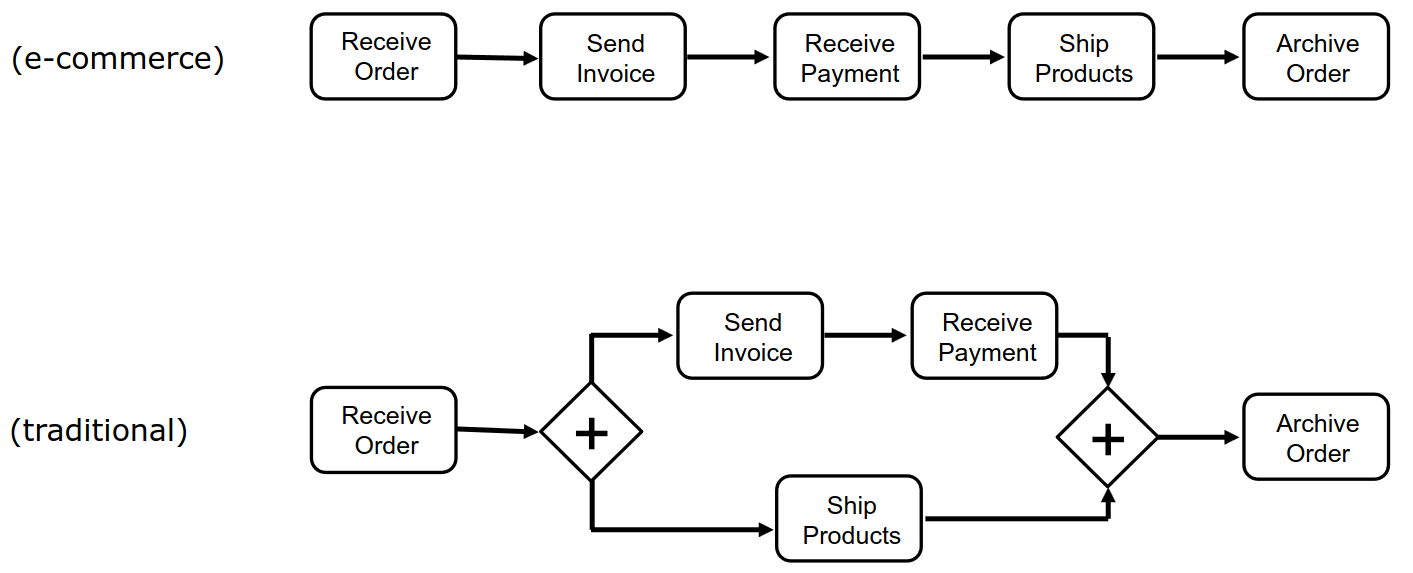
\includegraphics[width=0.95\columnwidth]{images/bp_activiesflow.png}
      \label{fig:bp_activiesflow}
   \end{figure}
\end{paracol}

\section{Notation for BPM}
\begin{figure}[htbp]
   \centering
   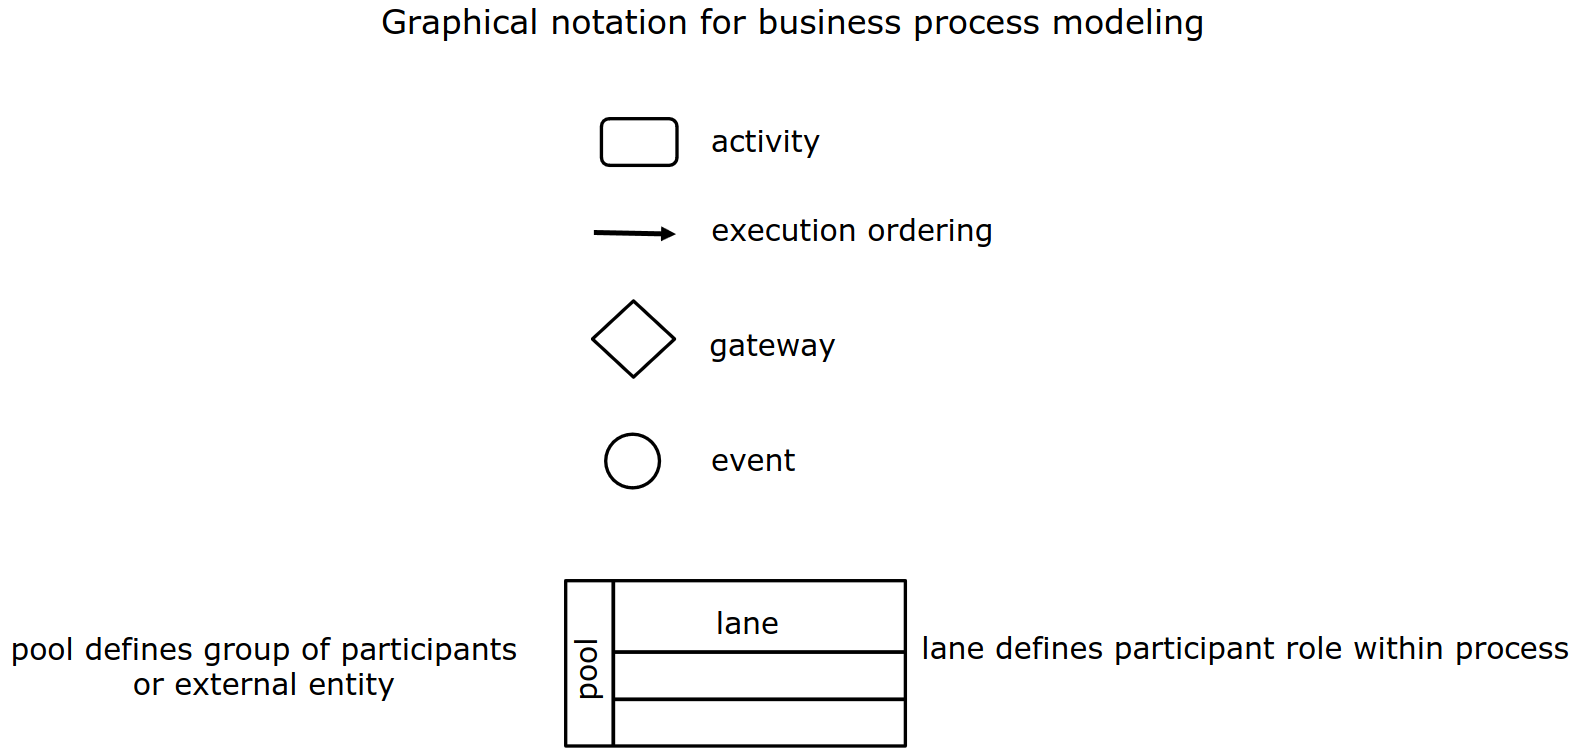
\includegraphics{images/bpm_notation.png}
   \caption{Business process model Notation}
   \label{fig:bpm_notation}
\end{figure}
Such notation is used as syntax to define BP models;
There are tools that support it and is deeply useful since \textbf{proving properties} of
business process models is a crucial aspect of business process management.

\begin{figure}[htbp]
   \centering
   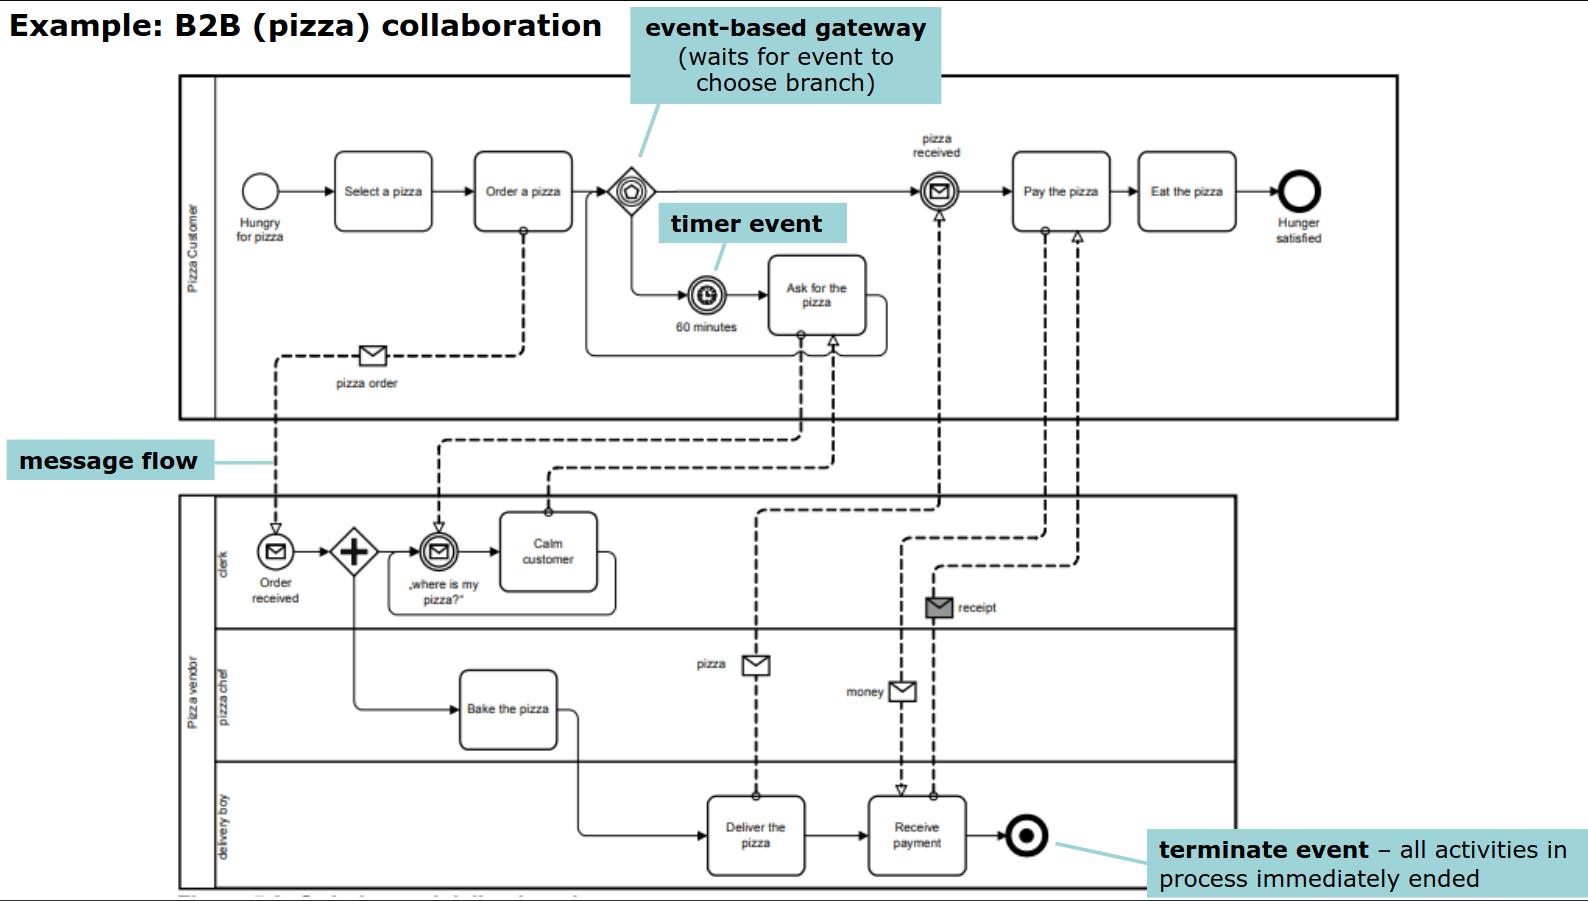
\includegraphics{images/bpm_pizza.png}
   \caption{Pizza BPM example}
   \label{fig:bpm_pizza}
\end{figure}

\section{Workflow Nets}
\textbf{Workflow Nets} are an extension of \textbf{Petri Nets}, and are one of the best known techniques for specifying business processes in a \textbf{formal} and \textbf{abstract} way.

\textit{Petri nets} consist of \textbf{places}, \textbf{transitions} and direct \textbf{arcs} connecting places and transitions.
Transitions model \textbf{\textit{activities}}, places and arcs model \textbf{\textit{execution constraints}}.
System dynamics are represented by \textbf{tokens}, whose distribution over the places
determines the \textit{state} of modelled system;
a transition can \textit{"fire"} if there is a \textit{token} for each of its input \textit{places}:
when it fires, one token is removed from each input place and one token is added to each input place.
\begin{figure}[htbp]
   \centering
   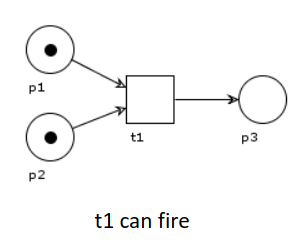
\includegraphics[width=0.225\columnwidth]{images/petri_firetoken1.png}
   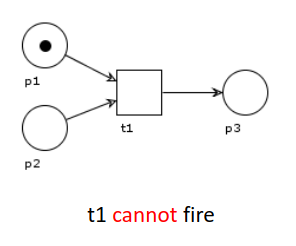
\includegraphics[width=0.225\columnwidth]{images/petri_firetoken2.png}
   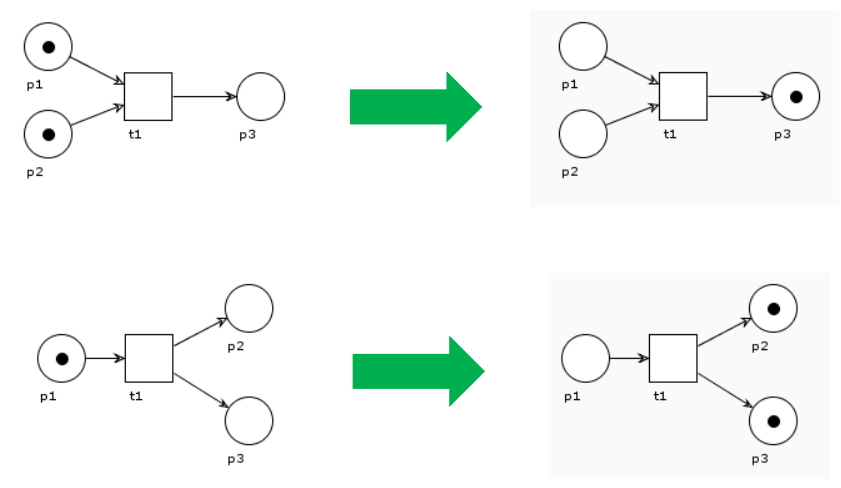
\includegraphics[width=0.45\columnwidth]{images/petri_firetoken3.png}
   \caption{Transition firing}
   \label{fig:petri_firetoken}
\end{figure}
\nl

A \textit{Petri net} is a \textbf{\textit{workflow net}} \texttt{iff}
\begin{enumerate}
   \item There is a \textit{unique \textbf{source} place} with no incoming edge
   \item There is a \textit{unique \textbf{sink} place} with no outgoing edge
   \item All places and transitions are located on some path from
   the initial place to the final place
\end{enumerate}

In workflow nets, there may be "sugared" explicit versions of \texttt{AND} and \texttt{OR},
and transitions may be annotated with triggers to indicate which entity is responsible for the transitions to fire.

\begin{figure}[htbp]
   \centering
   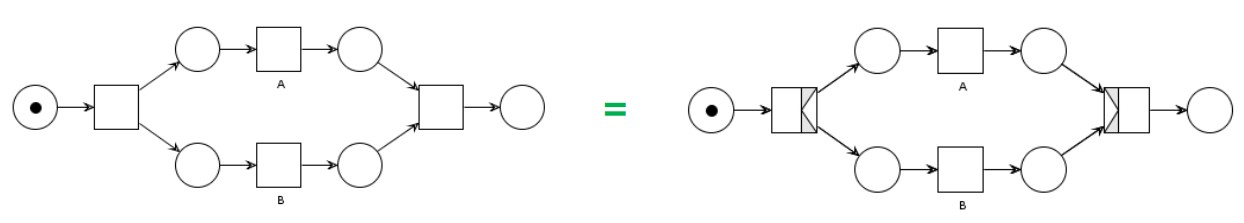
\includegraphics{images/wfnet_expland.png}
   \caption{Explicit \texttt{AND-split} and \texttt{AND-join} transitions}
   \label{fig:wfnet_expland}
\end{figure}
\begin{figure}[htbp]
   \centering
   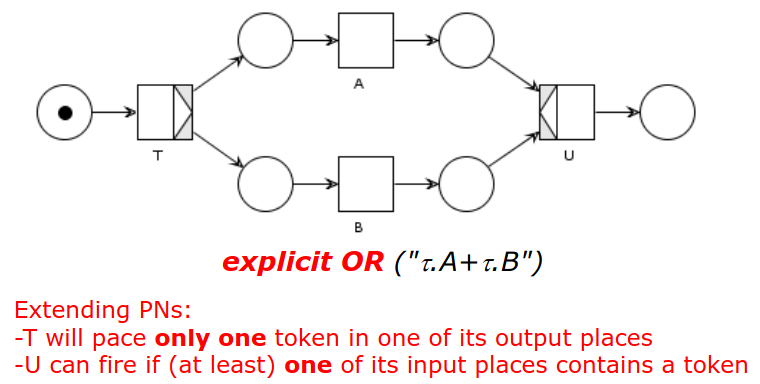
\includegraphics{images/wfnet_explor.png}  
   \caption{Explicit \texttt{OR}}
   \label{fig:wfnet_explor}
\end{figure}
\nl

\labelitemize{\textbf{Soundness}}{
   A workflow net is {--}unformally{--} \textbf{sound} \texttt{iff}:
   \begin{enumerate}
      \item every net execution starting from the initial state 
      eventually leads to the final state
      \note{
         Recall that:
         \begin{itemize}
            \item 
            \textbf{Initial state} - 
            one token in the sink place, no tokens elsewhere
            \item
            \textbf{Final state} - 
            one token in the source place, no tokens elsewhere
         \end{itemize}
      }
      \item every transition occurs in at least one net execution
   \end{enumerate}
}

\begin{figure}[htbp]
   \centering
   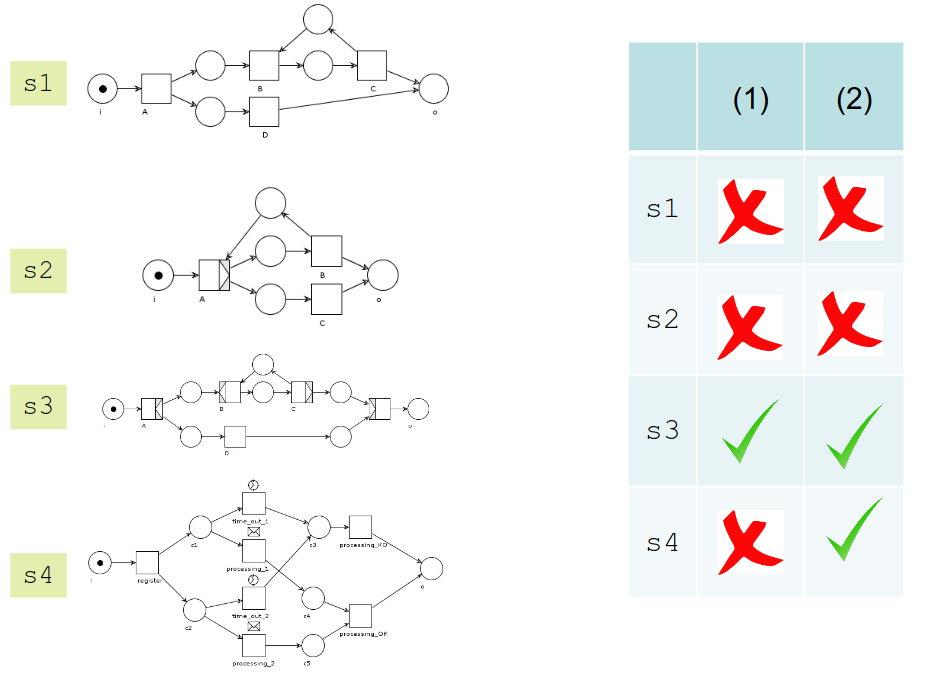
\includegraphics{images/wfnet_sound.png}
   \caption{Soundness check with examples}
   \label{fig:wfnet_sound}
\end{figure}

\subsubsection*{(More) Notation}
\begin{itemize}
   \item \Letter{} message activated
   \item \VarClock{} time activated
   \item \APLdownarrowbox{} user activated
\end{itemize}

\subsection{Formally}
A Petri net $(PN,M)$ is \textbf{live} $\Longleftrightarrow$ for any reachable state $M'$ and every transition $t$ there is a reachable state $M''$ reachable from $M'$ where $t$ is enabled.

\begin{figure}[htbp]
   \centering
   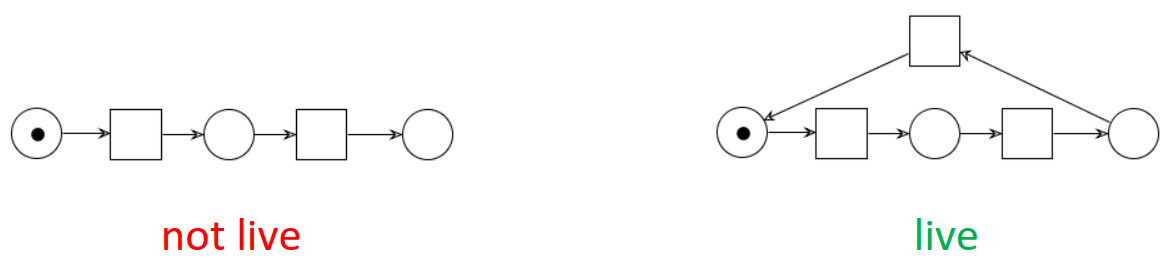
\includegraphics{images/wfnet_liveness.png}
   \label{fig:wfnet_liveness}
\end{figure}

A Petri net $(PN,M)$ is \textbf{bounded} $\Longleftrightarrow$ for each place $p$ there is an $n \in N$ such that for each reachable state $M'$ the number of tokens in $p$ in $M'$ is less than $n$.

\begin{figure}[htbp]
   \centering
   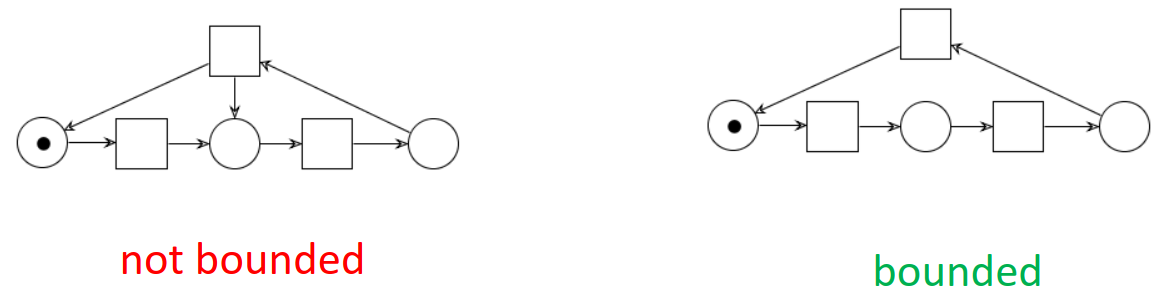
\includegraphics{images/wfnet_bounded.png}
   \label{fig:wfnet_bounded}
\end{figure}

\begin{theorem}   
   A worflow net $N$ is \textbf{sound} $\Longleftrightarrow$ ($\check{N}$,{i}) is both \textit{live} and \textit{bounded}, where $\check{N}$ is $N$ extended with a transition from the sink place $o$ to the source place $i$.
\end{theorem}
\subsection{BPMN to Workflow Nets}

\begin{figure}[htbp]
   \centering
   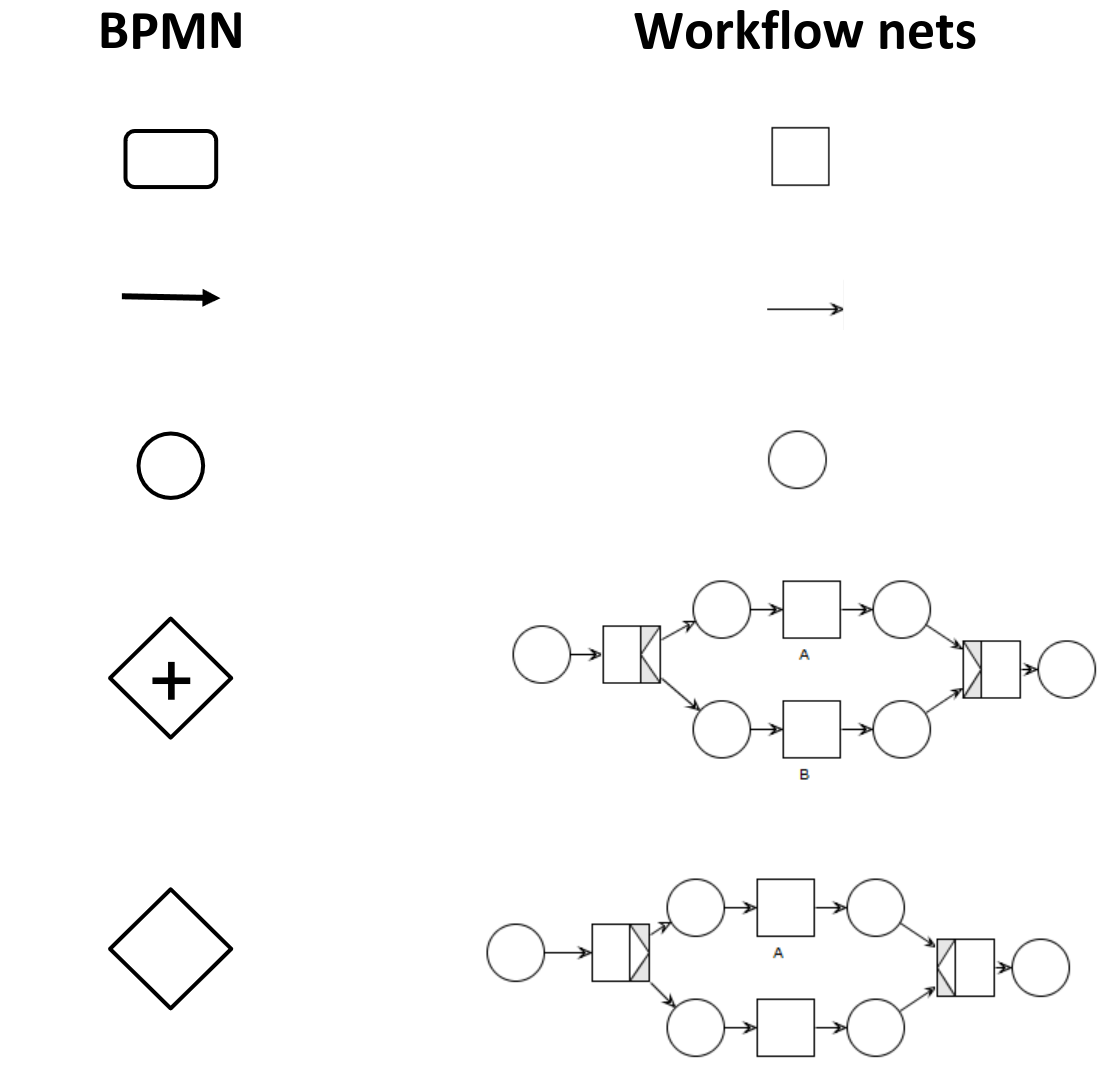
\includegraphics[width=0.5\columnwidth]{images/bpm_net1.png}
   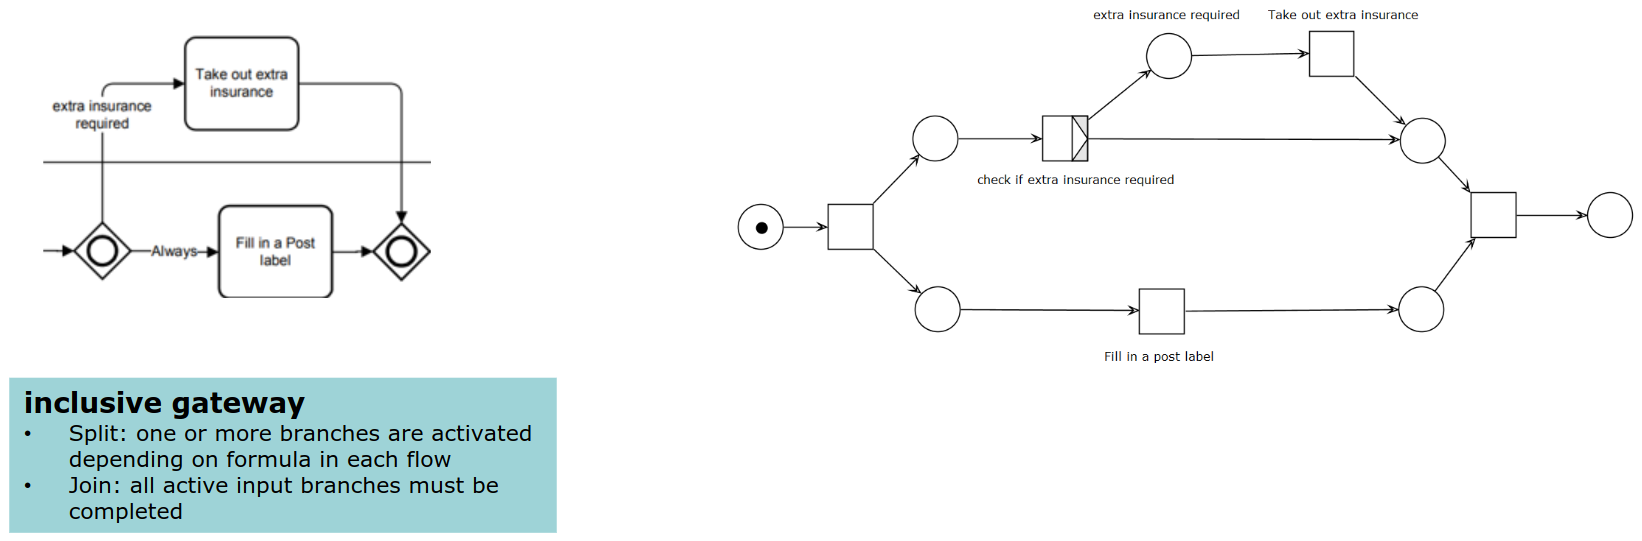
\includegraphics{images/bpm_net2.png}
   \caption{From BPMN to Workflow Nets}
   \label{fig:bpm_net}
\end{figure}